\textbf{4.1.} 电荷 Q 均匀地分布在半径为 R 的球体内，该球以匀角速度 $\omega$ 绕它的某个直径旋转，求球内离转轴为 r 处的电流密度的大小.

\vfill

\textbf{4.2.} 一条铝线的横截面积为 $0.10\mathrm{mm}^2$ ，在室温 $300\mathrm{K}$ 时载有 $5.0\times 10^{-4}\mathrm{A}$ 的电流.设每个铝原子有三个电子参与导电. 已知铝的原子量为 27, 室温下的密度为 $2.7 \mathrm{~g} \cdot \mathrm{cm}^{-3}$ , 电阻率为 $2.8 \times 10^{-8} \Omega \cdot \mathrm{m}$ , 电子的质量为 $m = 9.1 \times 10^{-31} \mathrm{~kg}$ , 阿伏伽德罗常数为 $6.0 \times 10^{23} \mathrm{~mol}^{-1}$ , 玻尔兹曼常量为 $k = 1.38 \times 10^{-23} \mathrm{~J} \cdot \mathrm{K}^{-1}$ . 求这条铝线内

(1) 电子定向运动的平均速率；

(2) 电子热运动的方均根速率；

(3) 一个电子两次相继碰撞之间的时间；

(4) 电子的平均自由程；

(5) 电场强度的大小.

\vfill

\newpage

\textbf{4.3.} 一段长为 $l$ 的圆台状导线，它的横截面积 $A$ 是 $x$ 的函数， $x$ 是到导线左端的距离，沿导线轴线的半截面形状示于习题4.3图。导线左端的横截面是半径为 $a$ 的圆，右端的横截面是半径为 $b$ 的圆，电导率 $\sigma$ 是常数。计算整段导线的电阻。

\begin{center}
    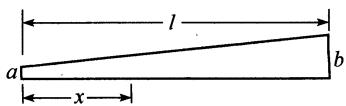
\includegraphics[width=0.3\linewidth]{figures/fig_4_4_1.jpg}
\end{center}
\vfill

\textbf{4.4.} 五个电阻按习题 4.4 图所示连接, 求 a、b 间的电阻.

\begin{center}
    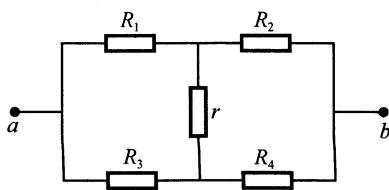
\includegraphics[width=0.3\linewidth]{figures/fig_4_4_2.jpg}
\end{center}

\vfill

\newpage

\textbf{4.5.} 在半径为 a、b 的同心球壳导体之间填满电导率为 $\sigma$ 的导电介质，求两球壳之间的电阻.

\vfill

\textbf{4.6.} 如习题 4.6 图所示的无限网格电路, 全部电阻的阻值相同, 设为 r, 求 A 和 B 之间的等效电阻 $R_{AB}$ .
\begin{center}
    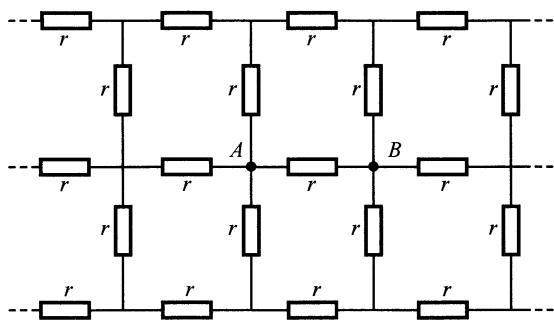
\includegraphics[width=0.3\linewidth]{figures/fig_4_6.jpg}
\end{center}

\vfill

\newpage

\textbf{4.7.} 甲乙两站相距 $50\mathrm{km}$ , 其间有两条相同的电话线, 有一条因某处触地而发生故障, 甲站的检修人员用习题 4.7 图中的办法找出触地处到甲站的距离 $x$ : 让乙站把两条电话线短路 (即接在一起), 接通电桥电路, 调节 $r$ 使通过检流计 $G$ 的电流为零. 已知电话线每千米长的电阻为 $6\Omega$ , 测得 $r = 360\Omega$ , 求 $x$ .

\begin{center}
    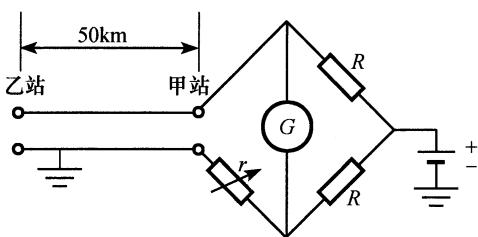
\includegraphics[width=0.3\linewidth]{figures/fig_4_8_1.jpg}
\end{center}
\vfill

\textbf{4.8.} 丹聂尔电池由两个同轴圆筒构成，长为 $l$ ，外筒是内半径 $b$ 的铜，内筒是外半径为 $a$ 的锌，两筒间充满介电常量为 $\varepsilon$ 、电阻率为 $\rho$ 的硫酸铜溶液，如习题4.8图所示.略去边缘效应，求

(1)该电池的内阻；

(2) 该电池的电容；

(3) 内阻与电容之间的关系.

\begin{center}
    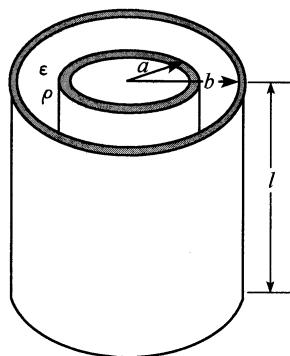
\includegraphics[width=0.2\linewidth]{figures/fig_4_8_2.jpg}
\end{center}

\vfill

\newpage

\textbf{4.9.} 如习题 4.9 图所示, 3 个电源的电动势分别为 $\mathcal{E}_{1}=12.0V, \mathcal{E}_{2}=\mathcal{E}_{3}=6.0V$ , 电阻 $R_{1}=R_{2}=R_{3}=3\Omega, R_{4}=6\Omega$ , 求 $R_{4}$ 上的电压和通过 $R_{2}$ 的电流.

\begin{center}
    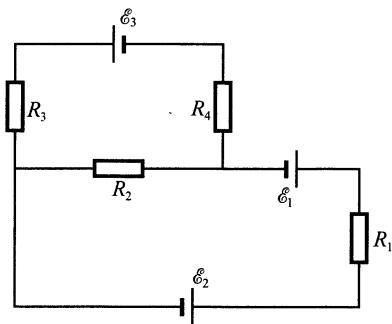
\includegraphics[width=0.3\linewidth]{figures/fig_4_10_1.jpg}
\end{center}
\vfill

\textbf{4.10.} 一直流电路如习题4.10图所示，其中， $\mathcal{E}_1 = 3\mathrm{V}, \mathcal{E}_2 = 1.5\mathrm{V}, \mathcal{E}_3 = 2.2\mathrm{V}; R_1 = 1.5\Omega, R_2 = 2.0\Omega, R_3 = 1.4\Omega$ ；电源的内阻不计，试求 $a, b$ 两点之间的电势差。

\begin{center}
    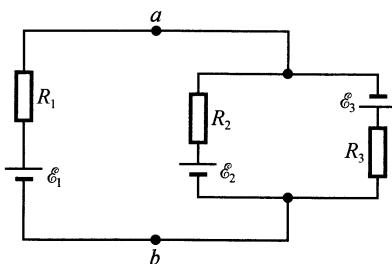
\includegraphics[width=0.3\linewidth]{figures/fig_4_10_2.jpg}
\end{center}

\vfill

\newpage

\textbf{4.11.} 一电路如习题4.11图所示. 已知 $\mathcal{E}_1 = 12\mathrm{V}, \mathcal{E}_2 = 10\mathrm{V}, \mathcal{E}_3 = 8\mathrm{V}, r_1 = r_2 = r_3 = 1\Omega, R_1 = R_3 = R_4 = R_5 = 2\Omega, R_2 = 3\Omega,$ 求

(1) 图(a)中 $a, b$ 两点间电压；

(2) 图(b)中通过 $R_{1}$ 的电流
\begin{center}
    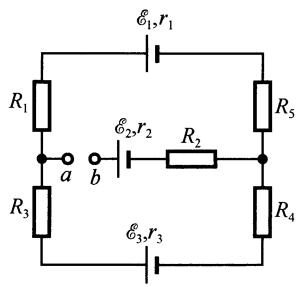
\includegraphics[width=0.3\linewidth]{figures/fig_4_12_1.jpg}
    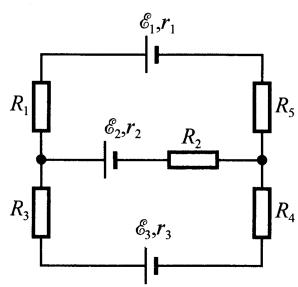
\includegraphics[width=0.3\linewidth]{figures/fig_4_12_2.jpg}
\end{center}
\vfill

\textbf{4.12.} 在习题 4.12 图所示电路中，已知： $E_{1}=6V, E_{2}=4.5V, E_{3}=2.5V, R_{1}=R_{2}=0.5\Omega, R_{3}=2.5\Omega$ ，忽略电源内阻，求通过电阻 $R_{1}, R_{2}$ 和 $R_{3}$ 的电流。
\begin{center}
    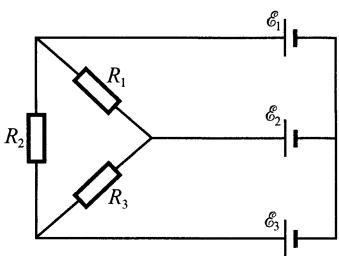
\includegraphics[width=0.3\linewidth]{figures/fig_4_12_3.jpg}
\end{center}

\vfill
\newpage


\textbf{4.13} 两同心导体球壳半径 $a < b$ ，球壳间充满电导率为 $\sigma$ 、介电常量为 $\varepsilon$ 的均匀介质。设 $t = 0$ 时刻内球壳带电 $q$ ，试求

(1) 介质中的传导电流强度的时间变化规律；

(2) 传导电流总共产生多少焦耳热。

\vfill

\textbf{4.14} 如习题 4.14 图所示,有半径分别为 $R_{1}$ 和 $R_{2}$ 的同轴导体圆筒,长为 $L(L \gg R_{1}, R_{2})$ . 设两筒间充满两层均匀介质，其分界面是与导体圆筒同轴的圆柱面，半径为 $R_0$ ，介质 $a,b$ 的介电常量分别为 $\varepsilon_{a}$ 和 $\varepsilon_{b}$ ，电导率分别为 $\sigma_{a}$ 和 $\sigma_{b}$ .在两筒间加上恒定电压 $U$ ，求

(1) 两导体圆筒间的电阻和电流；

(2) 各界面的自由电荷分布.
\begin{center}
    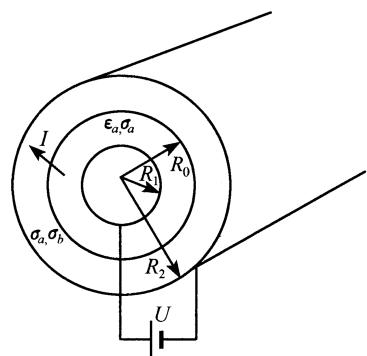
\includegraphics[width=0.3\linewidth]{figures/fig_4_12_4.jpg}
\end{center}

\vfill

\newpage

\textbf{4.15.} 将两个导体嵌入到电导率为 $10^{-4}\mathrm{S}\cdot \mathrm{m}^{-1}$ 、介电常量为 $\varepsilon = 80\varepsilon_0$ 的介质中，测得这两个导体之间的电阻为 $10^{5}\Omega$ ，计算这两个导体之间的电容.
